\section{Análisis Exploratorio de Datos}

Tras garantizar la integridad estructural del conjunto de datos y definir un espacio de características depurado, se procede a la fase de Análisis Exploratorio de Datos (EDA). El propósito de esta sección es analizar el comportamiento, la distribución y la dispersión de cada variable. Iniciaremos con un enfoque univariado permitiendonos comprender la naturaleza demográfica de las cohortes, la concentración del financiamiento en regiones específicas de México y las métricas financieras típicas que componen el mercado nacional.

\subsection{Análisis Univariado}

\subsubsection{Distribución de las Etapas de Riesgo}
Primeramente, necesitamos una comprensión absoluta de la variable objetivo (\texttt{etapa}). 

Las estadísticas descriptivos de la muestra (1,000,000 de cohortes) arrojan una distribución donde el 81.09\% se clasifica en Etapa 1 (riesgo bajo o al corriente), el 10.88\% en Etapa 2 (riesgo significativo o deterioro temprano) y el 8.03\% en Etapa 3 (riesgo alto, cartera vencida o en incumplimiento).

\begin{figure}[H]
	\centering
	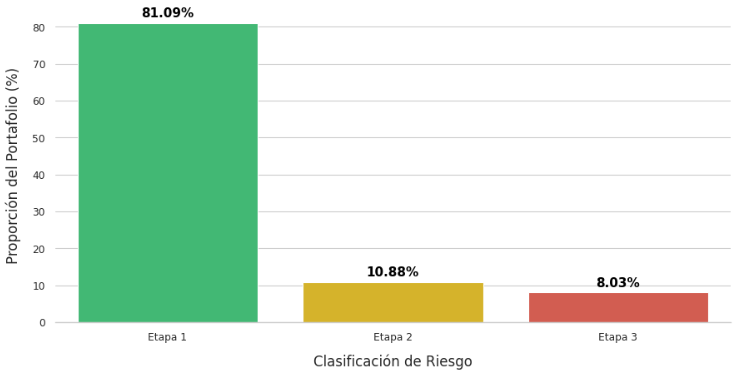
\includegraphics[scale=0.6]{imagenes/Capturas/graph-4-1.png}
	\vspace{0pt}
	\caption{Distribución de la variable \texttt{etapa}}
	\vspace{0pt}
\end{figure}

Esta distribución es esperable con la realidad del sector financiero; es indispensable para la viabilidad de las instituciones que la inmensa mayoría de la cartera se mantenga con un riesgo bajo, aplicando rigurosos filtros para evitar pérdidas. No obstante, un 18.91\% combinado de cartera con deterioro (Etapas 2 y 3) representa un volumen considerable crítico.
Esta proporción confirma la presencia de un \textit{desbalance de clases}. En consecuencia, la métrica de Exactitud (\textit{Accuracy}) queda descartada como criterio principal de evaluación. Un modelo predictivo ingenuo que clasificara a todas las cohortes en Etapa 1 obtendría un 81\% de exactitud, lo cual sería financieramente desastroso. Para la toma de decisiones institucionales, el costo de un Falso Negativo (evaluar una cohorte de alto riesgo como si fuera de riesgo bajo) es asimétricamente superior al de un Falso Positivo. Por tanto, el diseño de la red neuronal deberá priorizar la optimización de la Sensibilidad (\textit{Recall}) para la detección temprana de la cartera deteriorada.

\subsubsection{Distribución de las variables Financieras}
Las distribuciones de las masas monetarias muestran una alta asimetría positiva (\textit{Right Skewness}). Por ejemplo, el 75\% de las cohortes presentan un \texttt{monto\_originacion\_credito} igual o inferior a los \$4.2 millones de MXN; sin embargo, el límite superior alcanza cifras extremas de hasta \$3,151 millones de MXN. Como vimos en la detección de outliers, estas brechas gigantescas no constituyen errores, sino que reflejan realidades comerciales validas: cohortes masivas de miles de instrumentos hipotecarios o financiamientos de grandes desarrollos estructurales.  Por lo tanto, para una mejor visualización (sin el efecto visual de los outliers), se grafican las distribuciones en escala logarítmica.

Por otro lado, la \texttt{tasa\_ponderada} es la única variable que mantiene una estructura interpretable en escala lineal, con una media nacional del 10.31\% y una desviación estándar moderada del 1.91\%, presentando casos atípicos puntuales que escalan hasta el 36\% para esquemas de alto riesgo.

\begin{figure}[H]
	\centering
	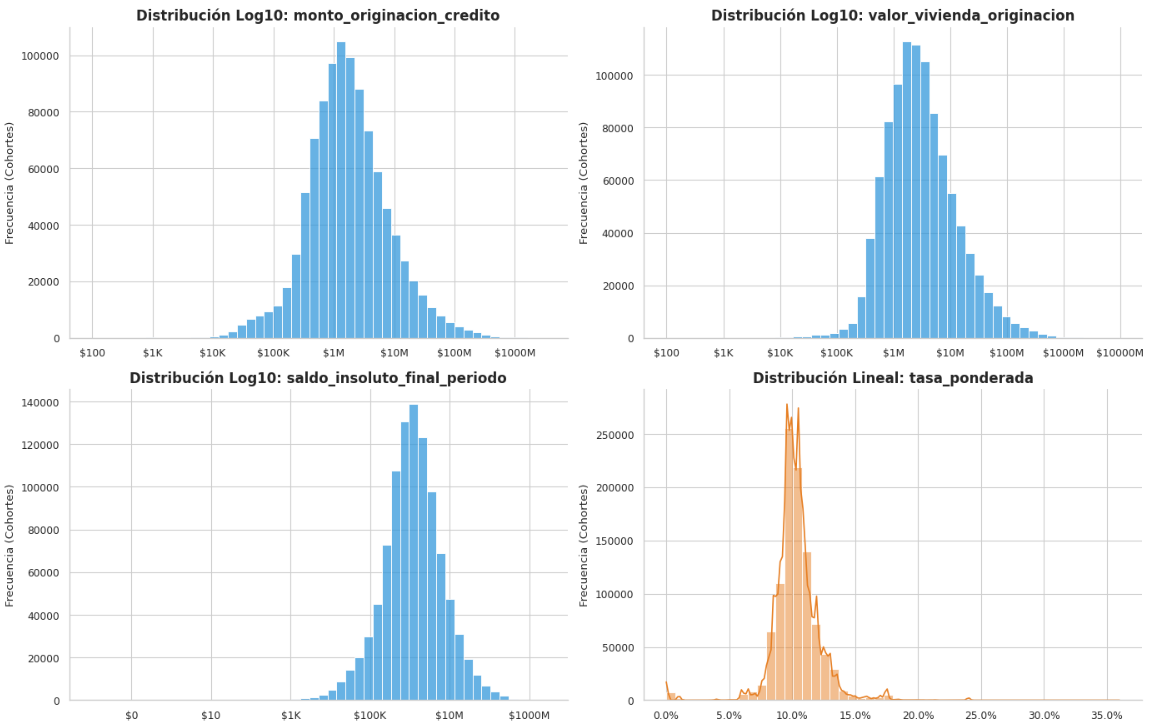
\includegraphics[scale=0.42]{imagenes/Capturas/graph-4-2.png}
	\vspace{0pt}
	\caption{Distribución de las variables financieras}
	\vspace{0pt}
\end{figure}

Para mitigar el efecto que estos valores extremos podrían inducir en los algoritmos sensibles a outliers, se corrobora la necesidad de aplicar transformaciones no lineales, como la transformación logarítmica o escaladores en la fase de preprocesamiento.

\subsubsection{Distribución de variables demográficas y socio-económicas}
El análisis de frecuencias de las variables categóricas revela una marcada concentración del portafolio en nichos poblacionales específicos:
\begin{itemize}
	\item Existe una concentración en los intervalos de edad de 36 a 45 años y de 46 a 55 años. Esto indica que el financiamiento hipotecario ocurre predominantemente en la mediana edad.
	\item Las cohortes financiadas se agrupan en los rangos de ingresos mensuales de \$20,001 a \$40,000 MXN y de \$40,001 a \$80,000 MXN. Esto evidencia que el mercado atiende principalmente a la clase media y media-alta.
	\item Una gran mayoría de las cohortes pertenece al Sector Privado (asalariados). Se identificó que las variables \texttt{tipo\_acreditado} y \texttt{sector\_laboral} proveen información redundante, justificando la eliminación de la primera para optimizar el espacio vectorial.
\end{itemize}

\begin{figure}[H]
	\centering
	\vspace{-10pt}
	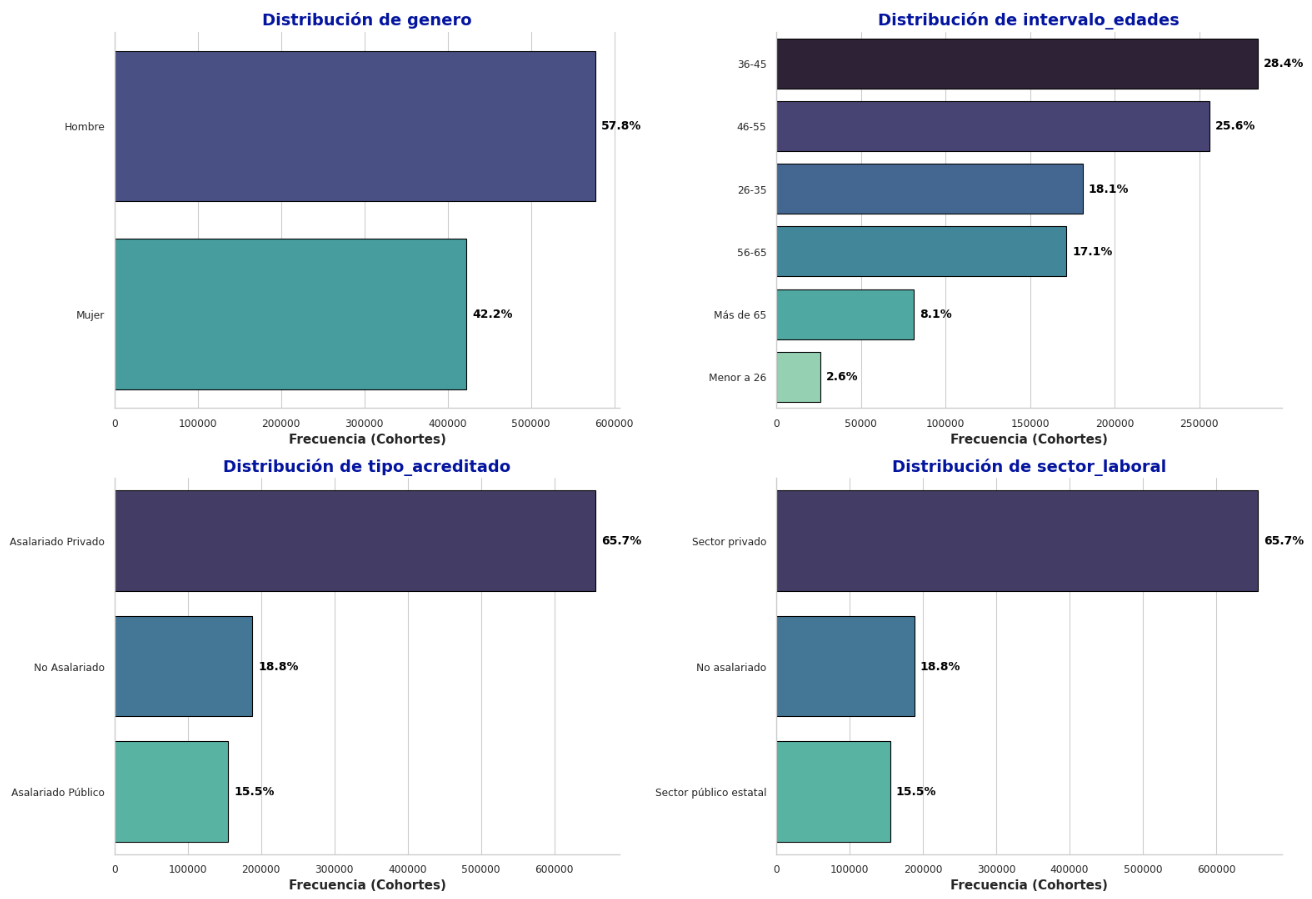
\includegraphics[scale=0.37]{imagenes/Capturas/graph-4-3.png}
	\vspace{-20pt}
\end{figure}
\begin{figure}[H]
	\centering
	\vspace{-10pt}
	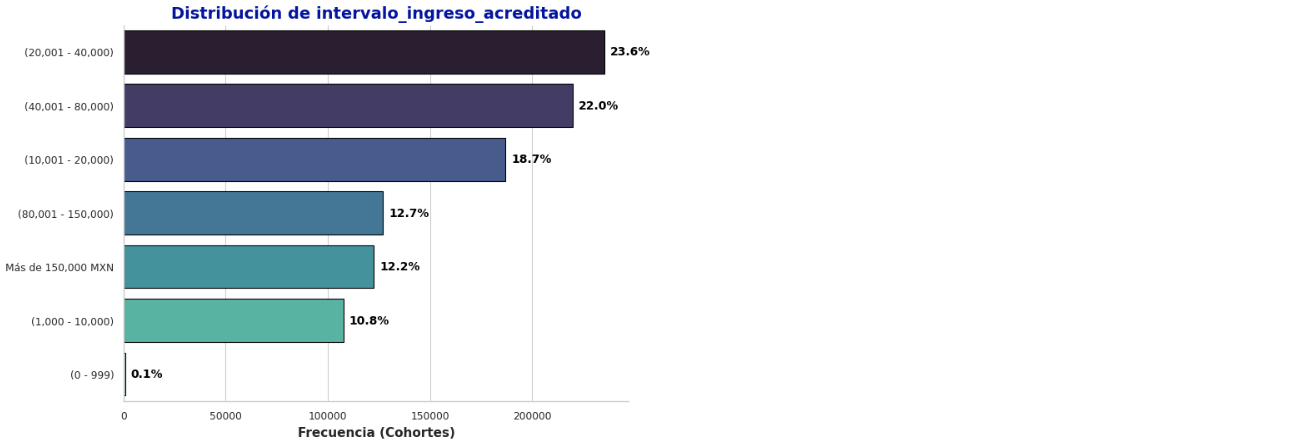
\includegraphics[scale=0.38]{imagenes/Capturas/graph-4-4.png}
	\caption{Distribución de las variables demográficas y socio-económicas}
	\vspace{-40pt}
\end{figure}

\subsubsection{Distribución de variables comerciales}
La naturaleza del activo en garantía y su localización geográfica también forman parte importante para alimentar a los modelos.
\begin{itemize}
	\item El crédito se centraliza en las regiones de mayor desarrollo industrial y económico del país: Ciudad de México (6.7\%), Jalisco (7.5\%) y Nuevo León (6.1\%).
	\item El portafolio se orienta fuertemente hacia la Adquisición de Vivienda Nueva (41.6\%) por encima de la vivienda usada (28.0\%). Asimismo, el 86.1\% de las cohortes se concentra en el segmento habitacional de nivel Medio o Residencial.
	\item La variable del nombre comercial del producto hipotecario exhibió una cardinalidad extrema (471 clases distintas), donde los 5 principales productos apenas consolidan el 21.95\% de la muestra. Esta fragmentación nos permite validar su exclusión del modelado predictivo al carecer de capacidad de generalización.
\end{itemize}

\subsubsection{Distribución de variables temporales e institucionales}
\begin{table}[H]
	\centering
	
	% Primera fila
	\begin{subtable}[t]{0.48\textwidth}
		\centering
		\caption{Periodo}
		\begin{tabular}{lrr}
			\toprule
			\textbf{Periodo} & \textbf{Frecuencia} & \textbf{\%} \\
			\midrule
			202504 & 40\,676 & 4.07 \\
			202411 & 40\,555 & 4.06 \\
			202502 & 40\,290 & 4.03 \\
			202508 & 40\,261 & 4.03 \\
			202506 & 40\,209 & 4.02 \\
			\vdots & \vdots & \vdots \\
			\bottomrule
		\end{tabular}
	\end{subtable}
	\hfill
	\begin{subtable}[t]{0.48\textwidth}
		\centering
		\caption{Sector}
		\begin{tabular}{lrr}
			\toprule
			\textbf{Sector} & \textbf{Frecuencia} & \textbf{\%} \\
			\midrule
			Banca Múltiple & 974\,696 & 97.47 \\
			Banca de Desarrollo & 16\,199 & 1.62 \\
			SOFOMER & 9\,105 & 0.91 \\
			\vdots & \vdots & \vdots \\
			\bottomrule
		\end{tabular}
	\end{subtable}
	
	\vspace{0.5cm}
	
	% Segunda fila
	\begin{subtable}[t]{0.48\textwidth}
		\centering
		\caption{Institución}
		\begin{tabular}{lrr}
			\toprule
			\textbf{Institución} & \textbf{Frecuencia} & \textbf{\%} \\
			\midrule
			Santander & 313\,014 & 31.30 \\
			Banorte & 187\,162 & 18.72 \\
			BBVA México & 155\,475 & 15.55 \\
			Scotiabank & 76\,672 & 7.67 \\
			HSBC & 75\,329 & 7.53 \\
			\vdots & \vdots & \vdots \\
			\bottomrule
		\end{tabular}
	\end{subtable}
	\hfill
	\begin{subtable}[t]{0.48\textwidth}
		\centering
		\caption{Moneda}
		\begin{tabular}{p{4.5cm} r r}
			\toprule
			\textbf{Moneda} & \textbf{Frecuencia} & \textbf{\%} \\
			\midrule
			Moneda Nacional (Pesos) & 978\,237 & 97.82 \\
			UDIS & 16\,303 & 1.63 \\
			VSMG (Veces Salario Mínimo General) & 5\,131 & 0.51 \\
			Dólares de E.E.U.U.A. & 329 & 0.03 \\
			\bottomrule
		\end{tabular}
	\end{subtable}
	\caption{Frecuencias de variables temporales e institucionales}
	
\end{table}
La distribución temporal resultó ser uniforme (aproximadamente un 4\% de los registros por cada mes reportado). Se explorará mejor en el análisis bivariado.

A nivel institucional, la Banca Múltiple consolida el 97.47\% de la cartera. Más aún, tan solo cinco instituciones acaparan más del 80\% de las cohortes hipotecarias a nivel nacional, lo que implica que las políticas de evaluación de estas entidades dictan la salud del mercado hipotecario. 

Finalmente, aunque el Peso Mexicano ejerce una hegemonía absoluta (97.82\%) sobre las demás divisas, estas otras divisas con volumen minoritario serán de importancia en el análisis bivariado.

% ============================================================

\subsection{Análisis Bivariado}

Tras estudiar el comportamiento individual de las variables, la segunda fase del Análisis Exploratorio de Datos consistió en evaluar las relaciones entre dos categorías, en particular su impacto directo sobre la variable objetivo. El propósito es identificar los predictores más robustos del deterioro crediticio y descartar aquellos que inyectan redundancia matemática al sistema.

\subsubsection{Correlación y Colinealidad en Variables Financieras}
En el modelado supervisado, la inclusión de atributos altamente correlacionados genera inestabilidad en los gradientes y aumenta innecesariamente el costo computacional. Para evaluar esta métrica, se calculó una matriz de correlación de Pearson sobre las variables monetarias continuas.

Los resultados confirmaron una colinealidad extrema ($|r| > 0.90$) entre la gran mayoría de las métricas de volumen. Por ejemplo, el coeficiente de correlación entre el saldo insoluto final y la masa de intereses generados alcanzó un 0.999. Paralelamente, el monto de originación del crédito y el valor de la vivienda presentaron un coeficiente de 0.949. Por consiguiente, esta exploración justifica la decisión de conservar exclusivamente el \texttt{saldo\_insoluto\_final\_periodo} como único indicador de volumen monetario y la \texttt{tasa\_ponderada} como indicador del costo del dinero, dada su independencia lineal frente a las métricas de volumen.

\begin{figure}[H]
	\centering
	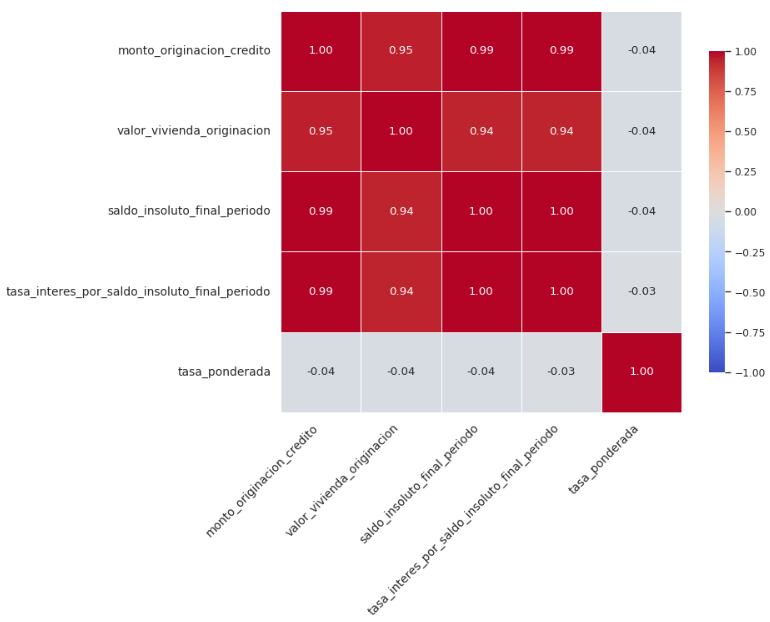
\includegraphics[scale=0.6]{imagenes/Capturas/graph-4-7.png}
	\vspace{0pt}
	\caption{Heatmap de correlación (Person) en variables financieras}
	\vspace{0pt}
\end{figure}

Al proyectar estas dos variables finales en diagramas de dispersión junto con una tercera dimensión de color (`etapa`), se evidenció la formación de nubes densas y bandas horizontales. Estas franjas reflejan la estandarización comercial de tasas fijas (del 9\%, 10.5\%, 11\%, etc.). La dispersión demostró que el riesgo no es linealmente separable mediante dos dimensiones continuas; las cohortes en Etapa 3 coexisten en los mismos rangos de tasa y saldo que las cohortes en Etapa 1, evidenciando que el incumplimiento es un fenómeno multidimensional.

\begin{figure}[H]
	\centering
	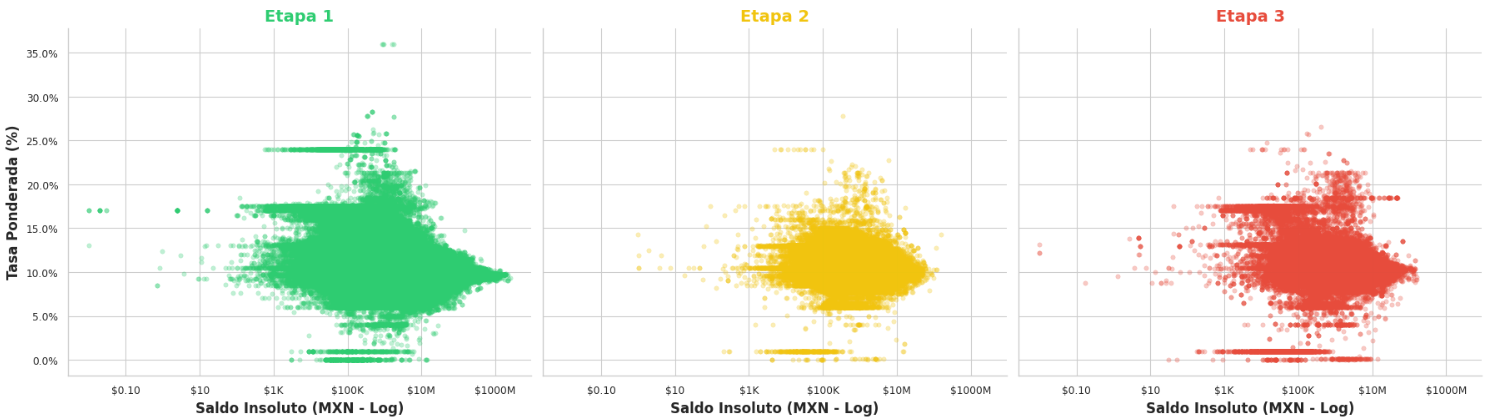
\includegraphics[scale=0.32]{imagenes/Capturas/graph-4-8.png}
	\vspace{0pt}
	\caption{Dispersión de saldo vs tasa de interés por etapas de riesgo}
	\vspace{0pt}
\end{figure}

\subsubsection{Dinámica de Riesgo: Variables catégoricas - Variable Objetivo}
Para cuantificar el impacto de los perfiles demográficos y comerciales sobre el riesgo, se definió la \textit{Tasa de Deterioro}. El Deterioro $D$ es la probabilidad condicional de que una cohorte transite hacia el riesgo significativo o alto $Y \in\{ \text{``Etapa 2''} \cup \text{``Etapa 3''}\}$, dado un atributo específico, $X = x_i$.:
$$
P(D \mid X = x_i) = \frac{\text{Frecuencia}(Y \in \{2,3\} \cap X = x_i)}{\text{Frecuencia}(X = x_i)}
$$
Calcular $P(D \mid X)$ nos permite identificar si una variable es útil para nuestro futuro modelo. Si la probabilidad de deterioro es demasiado similar en todas las categorías de $X$ (ej. hombres y mujeres incumplen exactamente igual), la variable no aporta información discriminante. Si la probabilidad cambia drásticamente, hemos encontrado un fuerte predictor de riesgo.

Se encontraron los siguientes hallazgos:
\begin{itemize}
	\item Los esquemas UDIS (28.18\% de deterioro) y Veces Salario Mínimo General o VSMG (29.37\%) exhiben tasas de incumplimiento muy superiores a las originaciones en Moneda Nacional (18.69\%), a pesar de que esta última predomina en las observaciones. Lo más destacado es que las obligaciones en Dólares presentaron la mayor tasa de deterioro (42.25\%), evidenciando se debe mantener a la divisa para evitar introducir sesgos en el entrenamiento.
	\item Las cohortes integradas por empleados del sector público poseen el riesgo más bajo del portafolio (10.83\%), en contraste con el sector privado (21.83\%).
	\item El riesgo de incumplimiento respecto a la edad no es lineal. Se concentra de manera acentuada en la adultez joven y madura: 36-45 años con un 21.73\% de deterioro, 26-35 años con 20.55\%, y 46-55 con 20.41\%, mientras que otros sectores más jovenes o en edad de vejez tienen una tasa aproximada de 14\%.
	\item Contrario a la intuición de una relación inversa (quien gana más está menos endeudado), la dinámica de ingreso-riesgo no es lineal. Los estratos medios-altos (ingresos de \$40,001 a \$150,000 MXN) resultaron ser los de menor riesgo (aprox 17\%). Los de mayores ingresos ("Más de \$150,000 MXN") y menos ingresos (10,001 - 20,000)  presentaron las más altas tasas de deterioro (21.21\%), aunque no hay que perder de vista qu esto puede sugiere un alto apalancamiento relativo en propiedades de inversión o de lujo (para los primeros), o bien, una gran densidad de individuos agrupados en una misma coherte (para los segundos).
	\item La adquisición de vivienda usada conlleva un riesgo de incumplimiento manifiestamente mayor (25.18\%) frente a la vivienda nueva (19.15\%). Esto puede estar asociado a imprevistos estructurales y costos de mantenimiento que comprometen la liquidez de los acreditados.
\end{itemize}

% [recordatorio para insertar gráficas de barra de la tasa de deterioro]

\subsubsection{Dinámica de Riesgo: Variables continuas - Variable Objetivo}
Al analizar la interacción entre las variables continuas y las etapas de riesgo mediante diagramas de caja (\textit{Boxplots}), se mostraron asimetrías importantes.

La mediana de los montos de originación para las cohortes de riesgo bajo (Etapa 1) es significativamente superior (\$1.7M) a la de las cohortes con deterioro o en incumplimiento (aprox \$1M). Como se explicó antes, el segmento de Interés Social (asociado a montos menores) aporta mayores tasas de incumplimiento que los montos mayores, ya que estos créditos exigen filtros más estrictos para evitar pérdidas severas para las instituciones, reduciendo su probabilidad de impago.

Por su parte, la mediana de la tasa ponderada asciende de forma suave conforme crece el nivel de riesgo (del 10.10\% en Etapa 1 al 10.50\% en Etapa 3). Este diferencial, aunque pequeño, indica que las instituciones logran identificar e manejar el riesgo relativo desde la originación, penalizando a las cohortes moroso con un costo de capital ligeramente superior (tampoco se pretende castigar excesivamente, para evitar agravar aún más la deuda).

\begin{figure}[H]
	\centering
	\vspace{-10pt}
	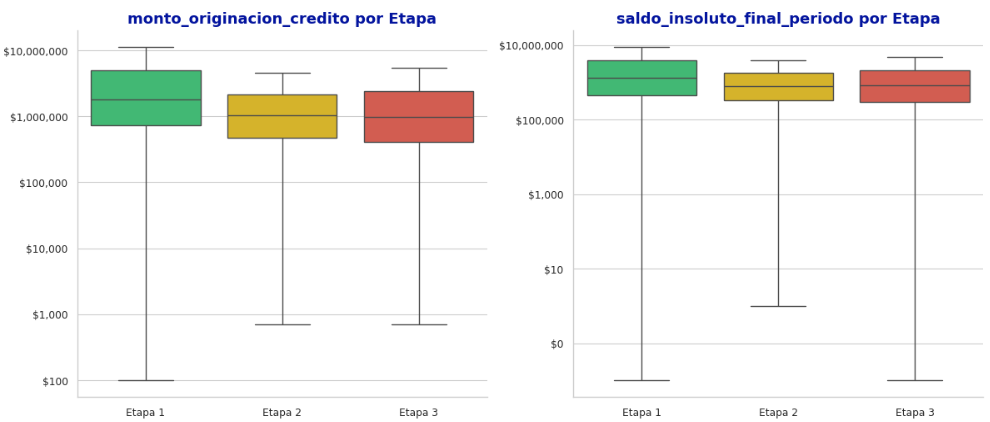
\includegraphics[scale=0.39]{imagenes/Capturas/graph-4-9.png}
	\vspace{-20pt}
\end{figure}
\begin{figure}[H]
	\centering
	\vspace{0pt}
	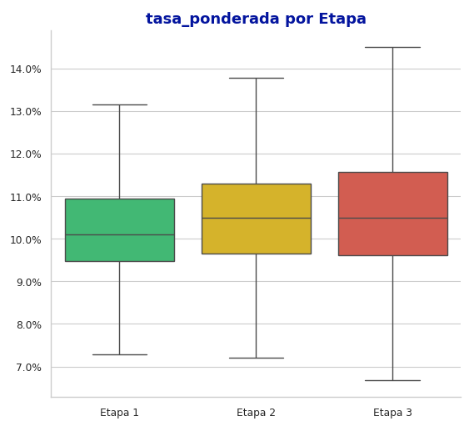
\includegraphics[scale=0.4]{imagenes/Capturas/graph-4-10.png}
	\caption{Boxplots de las variables financieras por etapas de riesgo}
	\vspace{-10pt}
\end{figure}

\subsubsection{Visualizaciones adicionales con Series de Tiempo}
El riesgo crediticio es un sujeto al tiempo, debido a las políticas monetarias y la pérdida de poder adquisitivo. Para concluir el análisis, se evaluó la evolución histórica de la Tasa de Deterioro a lo largo de los 25 meses disponibles en la muestra.

La serie de tiempo reveló una tendencia de deterioro gradual pero sostenida en el portafolio. En abril de 2024, el riesgo acumulado de las Etapas 2 y 3 se ubicaba en 18.28\%. Durante los siguientes 24 meses, la métrica experimentó un incremento escalonado hasta alcanzar un pico de 19.52\% a finales de 2025, estabilizándose en 19.36\% para el cierre del último mes reportado en abril de 2026. 

\begin{figure}[H]
	\centering
	\vspace{-10pt}
	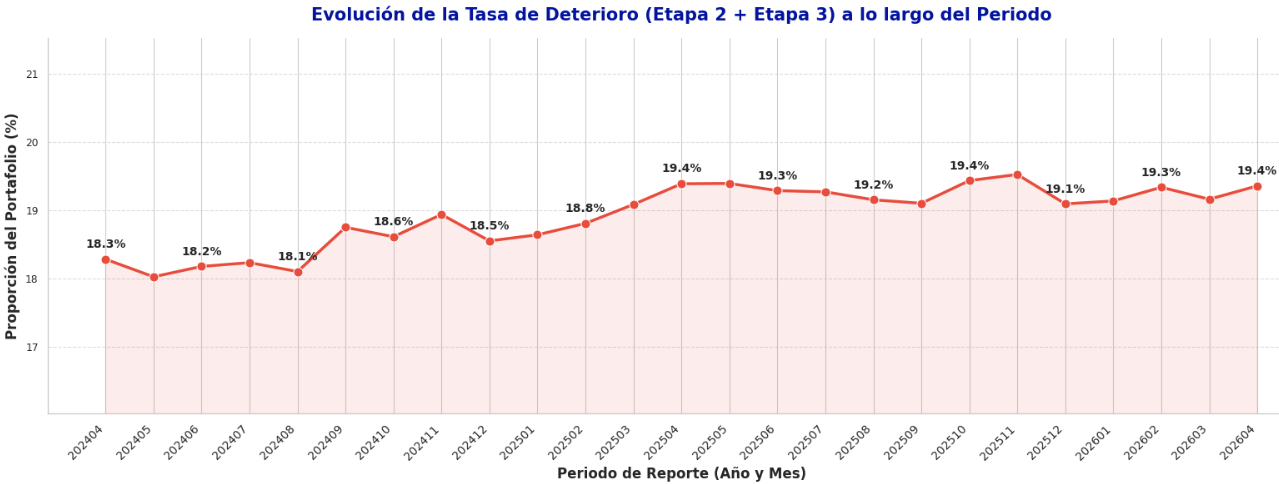
\includegraphics[scale=0.38]{imagenes/Capturas/graph-4-11.png}
	\caption{Serie de Tiempo de la Tasa de Deterioro}
	\vspace{-10pt}
\end{figure}

\subsection{Conclusiones y Selección de Características}
Concluida la exploración univariada y bivariada, se posee un entendimiento riguroso de las distribuciones y relaciones subyacentes en el conjunto de datos. Esto fue de vital importancia para justificar las decisiones presentadas en la sección \text{3.5. Reducción de Dimensionalidad y Selección de Características}.

Por lo que tras todo este proceso analítico, la dimensionalidad original de 20 columnas se redujo a un vector más manejable y altamente interpretable de 10 atributos esenciales: 
\begin{table}[H]
	\centering
	\begin{tabular}{r p{7cm} l}
		\hline
		& \textbf{Variable} & \textbf{Tipo de variable} \\
		\hline
		0 & \texttt{intervalo\_edades} & Categórica ordinal \\
		1 & \texttt{intervalo\_ingreso\_acreditado} & Categórica ordinal \\
		2 & \texttt{sector\_laboral} & Categórica nominal \\
		3 & \texttt{estado} & Categórica nominal \\
		4 & \texttt{destino\_credito} & Categórica nominal \\
		5 & \texttt{segmento\_vivienda} & Categórica nominal \\
		6 & \texttt{moneda} & Categórica nominal \\
		7 & \texttt{saldo\_insoluto\_final\_periodo} & Numérica continua \\
		8 & \texttt{tasa\_ponderada} & Numérica continua \\
		9 & \texttt{etapa} & Categórica ordinal \\
		\hline
	\end{tabular}
\end{table}
